\chapter{Model-based Approach to Estimate Gait Characteristics} \label{chapter:IMM}
The target population of this work is individuals with iSCIs, so the gait velocities of interest are very small in magnitude ($ \sim $ 0.5 m/s) \cite{nymark2005electromyographic}. There is limited work that uses physics-based models as a fundamental component in intent detection. The main attraction of using physics-based models is to allow for the accommodation of a greater number of users by modifying a small set of parameters such as mass, leg length, angles, and stiffness. This contribution uses the 3D B-SLIP model \cite{liu2015dynamic} as the basis of an estimation framework.

There are often physical changes to the gait as a result of changes in intended velocity, such as changes in step frequency, step length, and CoM trajectories \cite{kuo2001simple}. Template models emulate the salient characteristics of legged locomotion such as CoM trajectories and ground reaction force (GRF) profiles \cite{mochon1980ballistic}. Therefore, they may also emulate the changes in CoM trajectories and step length corresponding to changes in intent. The purpose of this contribution is to estimate gait characteristics such as gait phase and velocity through the comparison of sensor measurements to gaits from models of bipedal locomotion, specifically the B-SLIP model. The main idea behind the estimation framework developed is to estimate a person's desired gait velocity and phase by comparing the measured CoM trajectory to those in a library of B-SLIP gaits. 

User intent estimation may not necessarily be limited to forward velocity. Other aspects of intent changes not considered herein are the user's desires to initiate/terminate gait, change heading, and change gait mode i.e., transitions from walking on flat ground to ramps or stairs. In theory, the presented IMM framework may be extended to all these scenarios, with appropriate models of locomotion e.g., the B-SLIP model cannot describe gait initiation/termination. Considering multiple aspects of intent change for estimation at once may present difficulties as they may influence the gait differently and complicate the estimation problem via crosstalk. Considering only the gait velocity as a starting point helps break the estimation problem into a smaller subsection and reduces the challenges faced during estimation.

The challenges faced during estimation were the increased difficulty in finding low-speed periodic gaits during gait library generation and handling the hybrid dynamics of legged locomotion used to describe the different gait phases. The work done to address these challenges is described in this chapter. A linearization-based seed search method was developed to search for gaits at low walking speeds (less than 0.8 m/s). Additionally, Interacting Multi-Model (IMM) estimation was used to handle hybrid dynamics along with the library gaits. This chapter describes the results reported in a previous conference publication \cite{karulkarapplication}.

\section{Generating the gait library using the B-SLIP model}

Qualitative differences in the CoM trajectories of humans walking at different were observed in experimental data. Namely, the vertical and lateral excursion of the CoM over each step increase as gait velocity decreases. It was hypothesized that gait parameters may be estimated based on the changes in CoM trajectories. The 3D B-SLIP model presents a balance between model simplicity and CoM trajectory emulation. Additionally, using the 3D B-SLIP model allows the modeling of two important attributes of walking at low speeds; the lateral CoM movement that becomes increasingly dominant as gait velocity decreases and the DS period that represents a majority of the gait cycle. As the B-SLIP is a passive model, the omission of an actuator simplifies the estimation problem by reducing the assumptions necessary while applying these models to human walking. 

As described in Section~\ref{sec:bslip_model}, the state vector representing the CoM is $ \x_{CoM} = \left[x_{CoM} ,y_{CoM} ,z_{CoM} ,\dot{x}_{CoM} ,\dot{y}_{CoM} ,\dot{z}_{CoM}\right]^T $. The remaining parameters of the model, leg angles and stiffness, are collected in a parameter vector $ \greekvec{\zeta} = [\phi, \theta ,k ,z_{0_{CoM}} ,y_{0_{CoM}} ,\dot{x}_{0_{CoM}}]^T $ where $ \theta $ and $ \phi $ are leg angles that govern step length and width, and variables $ z_{0_{CoM}}$, $y_{0_{CoM}}$, and $\dot{x}_{0_{CoM}} $ give the vertical position, lateral position, and forward velocity of the CoM relative to the stance foot at the beginning of the step. The lack of actuators means optimization methods must be used to find periodic gaits for the B-SLIP model. An optimization procedure was carried out to find the parameters that would yield a fixed point for an MS-to-MS Poincar\'e map.

\subsection{Gait Optimization}
%
\begin{table}
	\centering
	\caption{Components of the gait optimization cost function \label{table:cost}}
	\small
\begin{tabular}{|c|m{0.7\linewidth}|}
	\hline
Cost component	& \multicolumn{1}{c|}{Description} \\
	\hline
$ z_{0_{CoM}} - z_{MDS} $	& Residual between CoM height at MS and Mid-Double-Support (MDS) to minimize vertical excursion. \\
	\hline
$ y_{0_{CoM}} - y_{foot_A} $	& Minimize distance of CoM ground projection to foot at MS. \\
	\hline
$ l_{step_{des}} - l_{step} $	& Residual between desired and actual step length. \\
	\hline
$ w_{step_{des}} - w_{step} $	& Residual between desired and actual step width. \\
	\hline
\end{tabular}




%\begin{eqnarray}
%	l_{step_{des}} &-& l_{step} \\
%	w_{step_{des}} &-& w_{step} \\
%	z_{0_{CoM}} &-& z_{MDS} \\
%	y_{0_{CoM}} &-& y_{foot_A}
%\end{eqnarray}
%
%$ g(\xi) $ are nonlinear constraints that ensure periodicity of the gait. 

\end{table}
%

Gait optimization was considered via a nonlinear programming problem
%
\begin{eqnarray}
	\min_{\greekvec{\xi}}& \quad \lVert{\mat{J}(\greekvec{\xi})}\rVert ^2 + (k_{max} - k) \label{eq:gaitOpt}\\
	\textrm{s.t.}& \quad \vec{g}(\greekvec{\xi}) \leq \epsilon \nonumber
\end{eqnarray}
%
where $ \mat{J}(\greekvec{\xi}) $ was a vector-valued function returning the vertical excursion of the CoM, deviation from a desired step length and width, and the distance from the ground projection of the CoM to the foot at MS with the equations listed in Table.~\ref{table:cost}. This cost function was designed to optimize periodic gaits that qualitatively resemble human walking. It was found that gaits optimized using periodicity as the sole criterion showed lower lateral and higher vertical CoM excursion than what was observed for human walking resulting in narrow step widths and step lengths. These factors resulted in CoM trajectories that did not resemble human walking. 

To ensure resemblance to CoM trajectories seen in humans, a penalty was added on the maximum vertical excursion of the CoM to flatten the trajectory in the sagittal plane. Secondly, since the mass loaded onto the spring is essentially in free-fall during SS1, the distance of the CoM from the stance foot was penalized to encourage more lateral excursion during SS1. The increased lateral excursion was further encouraged by driving leg stiffness toward an upper limit with the inclusion of $ (k_{max} - k) $ in the cost. Additionally, values for desired step length and width were included in the cost function to better emulate human walking.

The desired step length and width components of the cost were found to be critical for the convergence of the optimization. Step length $ l_{step} $ and width $ w_{step} $ depend on gait speed \cite{andriacchi1977walking}. These quantities were approximated as polynomial functions of the target gait velocity $ v_x $ with initial CoM height as a proxy for leg length, such that
\begin{eqnarray}
	l_{step} &=& [1\ v_x\ v_x^2\ z_{0_{CoM}} v_x] \greekvec{\gamma}_l \\
	w_{step} &=& [1\ v_x\ v_x^2\ z_{0_{CoM}} v_x] \greekvec{\gamma}_w
\end{eqnarray}
%
where $ \greekvec{\gamma}_l $ and $ \greekvec{\gamma}_w $ are the coefficients for step length and width respectively computed by fitting to human walking data of people under the age of 40 for treadmill and overground walking. The RMS error for this polynomial fit was approximately 3 cm for both, step length and width which was lower than the standard deviation of the measured data which was 9.7 cm and 3.4 cm respectively.

Nonlinear constraint functions $ \vec{g}(\vec{\xi}) $ ensured the periodicity of the gait by matching the initial and final positions and velocities of the CoM with respect to the trailing foot to a tolerance $ \epsilon $ (Table.~\ref{table:const}). 
%
\begin{table}
	\centering
    \caption{Nonlinear constraints for gait optimization\label{table:const}}
	\small
\begin{tabular}{|c|m{0.7\linewidth}|}
	\hline
	Constraint	& \multicolumn{1}{c|}{Description} \\
	\hline
	$ (x_{foot_A} - x_{f_{CoM}})^2 $	& Match distance of CoM ground projection to foot at MS. \\
	\hline
	$ (\dot{x}_{0_{CoM}} - \dot{x}_{f_{CoM}} )^2 $	&  Match initial and final forward velocity of the CoM. \\
	\hline
	$ (z_{0_{CoM}} - z_{f_{CoM}})^2 $	& Match initial and final vertical velocity of the CoM. \\
	\hline
	$ \dot{y}_{f_{CoM}}^2 $ & Ensure CoM has no lateral velocity at MS \\
	\hline
\end{tabular}

%\begin{eqnarray}
%	(z_{0_{CoM}} &-& z_{f_{CoM}})^2 \\
%	(x_{foot_B}) &-& x_{f_{CoM}})^2 \\
%	(y_{foot_B}) &-& y_{f_{CoM}})^2 \\
%	(\dot{x}_{0_{CoM}} &-& \dot{x}_{f_{CoM}} )^2\\
%	&\dot{y}_{f_{CoM}}^2
%\end{eqnarray}
\end{table}
%

As speed decreased, it was progressively difficult to choose appropriate parameters to seed the optimization, as the sensitivity of the model to initial conditions increased due to low passive stability at low speeds \cite{kuo2001simple}. This was an important challenge to overcome as gait speeds during rehabilitation are low \cite{seethapathi2015metabolic}. A predictor-corrector scheme was applied to start at a high-speed gait and compute appropriate seeds for low-speed gaits. 

\subsection{Linearization-based Seed Search}

\begin{figure}
	\centering
	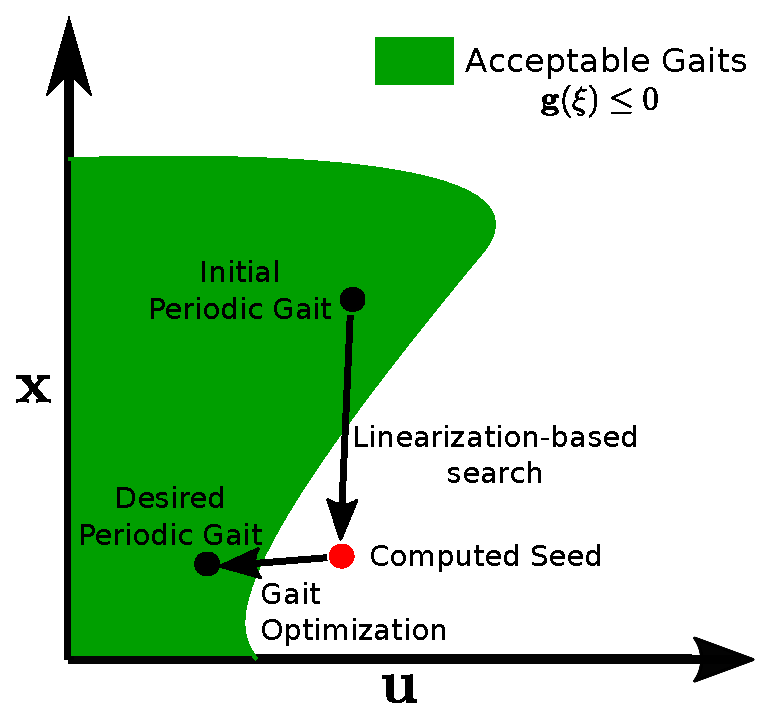
\includegraphics[width=0.5\linewidth]{homotopy.eps}
	\caption{Illustration of the linearization-based predictor-corrector search scheme to find periodic low-speed gaits}\label{fig:homotopy}
\end{figure}

Empirically, gaits at speeds greater than 0.8 m/s were found directly through optimization of \eqref{eq:gaitOpt} without special attention to initial seeds. A predictor-corrector strategy (Fig.~\ref{fig:homotopy}) was employed to address the challenges for lower velocities. In this strategy, an MS-to-MS Poincar\'e return map was linearized and used to solve for a preliminary seed during a homotopy process toward a lower-speed gait. This map is described by
%
\begin{equation}
	\x_{k+1} = \mathcal{P}(\x_k ,\u_k)
\end{equation}
%
where $\x_k$ denotes the state at MS and $\u_k$ denotes the discrete controls applied over one step as given by
\begin{align}
	\x &= \left[y_\com,\ z_\com,\ \dot{x}_\com,\ \dot{y}_\com\right]^T &
	\mathbf{u} &= \left[\phi,\ \theta,\ k\right]^T
\end{align}
The vertical velocity satisfies $\dot{z}=0$, the guard condition described in \eqref{eq:gms},  at MS. Thus $\dot{z}$ is omitted from the state $\x_k$ on the Poincar\'e surface. Following the optimization of one step of a periodic gait with state and control $\x^*_k$, $\u^*_k$, the return map is linearized providing
%
\begin{equation}\label{eq:linearized}
	\x_{k+1} \approx \x_{k+1}^* + \underbrace{\left.\frac{\partial \mathcal{P}}{\partial \x}\right|_{\x^*_k, \u^*_k}}_{:=\A} \delta \x_k + \underbrace{\left. \frac{\partial \mathcal{P}}{\partial \u}\right|_{\x^*_k, \u^*_k}}_{:=\B} \delta \u_k 
\end{equation}
%
where $\x_{k+1}^* = \mathcal{P}(\x_k^*, \u_k^*)$, $\delta \x_k = \x_k - \x^*_k$, and $\delta \u_k = \u_k - \u^*_k$. Since a gait of the 3D B-SLIP model is two-step periodic, left/right symmetry from step to step requires that $\x_{k+1}^* = \mathbf{S} \x_k^*$ where $\mathbf{S} = {\rm diag}([-1, 1, 1, 1])$. This matrix encodes that only the $y$-position of the CoM relative to the foot must change signs from step to step. Then, to solve for an approximate state/control pair for a lower-speed gait, variations to the parameters were found such that $\delta \x_{k+1} = \mathbf{S} \delta \x_k $. This constraint requires
\begin{align}\label{eq:linEq}
	\mathbf{0} = (\A-\mathbf{S})\delta \x_k + \B\delta \u_k\,. 
\end{align}

\begin{figure}
	\centering
	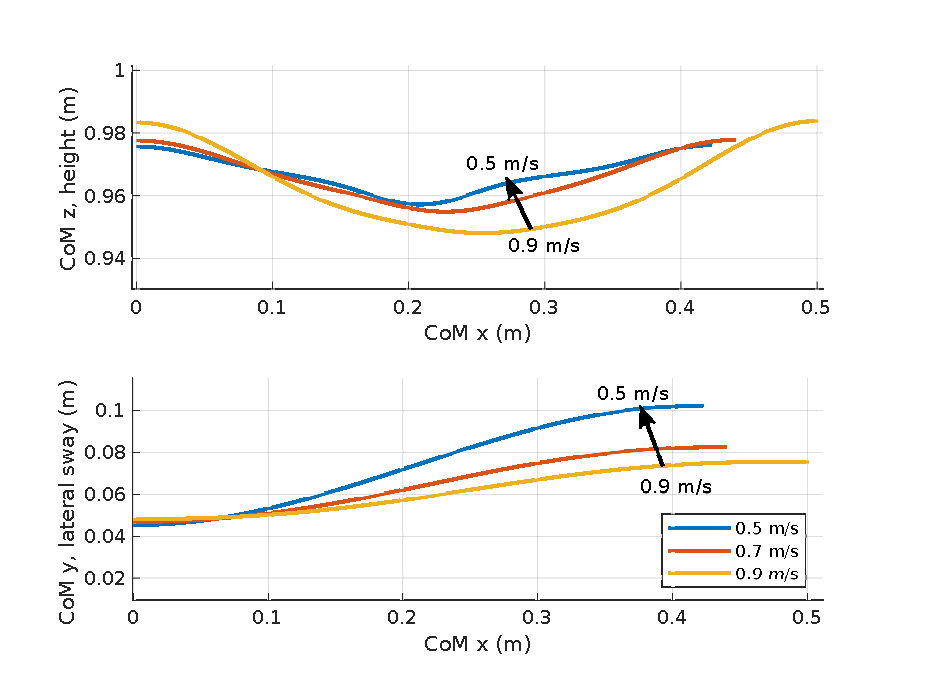
\includegraphics[width=0.7\linewidth]{subplot.eps}
	\vspace{-1em}
	\caption{A subset of the CoM trajectories in the gait library after optimization.}\label{fig:library}
\end{figure}

To generate a suitable next seed, the forward velocity component of $ \delta \x_k$ was held constant to the desired change in velocity. Considering \eqref{eq:linEq}, these equations provide 4 constraints for the 6 remaining unknowns, $ \left[\delta y_\com,\ \delta z_\com,\ \delta\dot{y}_\com,\ \delta \phi,\, \delta \theta,\, \delta k\right]^T  $, resulting in 2 degrees of freedom. Perturbations $\delta \x_k$ and $\delta \u_k$ satisfying these equations were computed with a least-norm solution, and the resulting parameters were used to seed the next gait optimization. This homotopy process was repeated until the desired low-velocity gait was optimized, resulting in a library of gaits for a range of speeds. Two libraries were generated: one at 0.4\,m/s - 0.9\,m/s for use with B-SLIP data and another at 0.6\,m/s - 1.0\,m/s for use with exoskeleton measurements, both at increments of 0.1\,m/s. As illustrated in Fig. \ref{fig:library}, generated libraries qualitatively exhibit the vertical and lateral CoM excursion trends that are observed in human data. That is vertical excursion decreases, and lateral excursion increases with a decrease in forward velocity. This linearization-based gait search method makes the generation of low-speed gaits easier and yields a library that serves as the basis for the IMM estimator outlined in the next section.

\section{Interacting Multi-Model Estimation}

\begin{figure}
	\centering
	\begin{overpic}[width=0.8\linewidth,percent]{IMMblock2.pdf}
		\put(48.5,6){\textbf{\scriptsize{Eq.\eqref{eq:physicalLikelihood}},}}
		\put(52.5,3){\textbf{\scriptsize{\eqref{eq:weightCalc}}}}
		\put(72,4){\textbf{\scriptsize{Eq.\eqref{eq:estimates},\eqref{eq:covFuse}}}}
		\put(72,36){\textbf{\tiny{Eq.\eqref{eq:updatex}-\eqref{eq:updateP}}}}
	\end{overpic}
	\caption{IMM scheme used to estimate gait phase and walking speed.}\label{fig:IMM}
\end{figure}
The IMM is a technique to  adaptively fuse estimates from multiple filters, running in parallel. Despite their use in other hybrid systems (\cite{bar2005imm},\cite{daeipour1998imm}), the application of IMMs to legged locomotion has been minimal. One example is the use of IMMs for legged locomotion is in state estimation and gait phase prediction for RHex \cite{skaff2005context}, a six-legged robot with compliant legs. Gait phase estimation is possible by directly using force
sensors in the exoskeleton soles \cite{agostini2013segmentation,de2012gait}. However, by relating human data to template models, the presented approach may provide insight into unmeasured parameters, such as leg stiffness, and the effects of changes in them on the gait.

The IMM estimation process used in this work is illustrated in Fig. \ref{fig:IMM}. Each of the $M$ filters represents a different candidate gait and phase, and the IMM attempts to determine which of the phases is most likely. 
In what follows, $ i $ and $ j $ index over filters, and $ k$ indexes over time. There are two types of estimate interactions shown in Fig.~\ref{fig:IMM}. First, a likelihood-based mixing produces an ensemble estimate output from the IMM, while a Markov mixing relates the state estimates from the filters at time step $k$ to the initial estimates at time step $k+1$. 

The filters begin with initial state estimates $\fsup{\xh_k^0}{j}$ and covariances $\fsup{\P_k^0}{j}$ that are propagated forward to $\fsup{\xh_k^-}{j}$ and $\fsup{\P_k^-}{j}$ using the dynamics presented in Eq.~\eqref{eq:sysProp} and~\eqref{eq:covProp}. Measurements from the exoskeleton sensors are used to initialize the filter at start-up and the covariance is set to be an identity matrix. The measurement likelihood ${}^j  \ell_k$ is then calculated for the state estimate of each filter as
\begin{align} \label{eq:likelihood}
	{}^j \ell_k &= p(\yt_k|\fsup{\xh_k^-}{j})  = {\rm det}( 2 \pi \fsup{\E_k}{j})^{-1/2} \,  {e}^{\lambda_r} \,~\textrm{where}\\[.5ex]
	\lambda_r &= -\frac{1}{2}\ {}^j\e_k^T \, \fsup{\E_k^{-1}}{j} \, \fsup{\e_k}{j} \nonumber
\end{align}
and $ \fsup{\e_k}{j} $ and $ \fsup{\E_k}{j} $ denote the measurement residual and its covariance, respectively, given by $ \fsup{\e_k}{j} = \yt_k - \h\!\left( \fsup{\xh_k^-}{j}\right)$ and 
\[
\fsup{\E_k}{j} = \fsup{\H_k}{j}\ \fsup{\P_k^{-}}{j}\ \fsup{\H_k^T}{j} + \fsup{\R_k}{j}. \] 
with $\fsup{\H_k}{j}$
the Jacobian of the measurement function at $\fsup{\xh_k^-}{j}$.

The measurement likelihood is then normalized across the $M$ models to calculate model weights $\fsup{w_k}{j}$ via
\begin{eqnarray}
	\fsup{w_k}{j} =  \fsup{ \ell_k}{j} \left/ \left( \textstyle\sum_{i=1}^{M} \fsup{ \ell_k}{i} \right) \right. \label{eq:weightCalc}
\end{eqnarray}
The magnitude of the weight $\fsup{w_k}{j}$ indicates the relative confidence of the filter that the system is in mode $j$ at time step $k$. In contrast to a conventional IMM approach \cite{Crassidis} where $\fsup{w_k}{j} = \fsup{w_{k-1}}{j} p(\yt_k|\fsup{\xh_k^-}{j})$, the weights from the previous iteration are not included in \eqref{eq:weightCalc}. This change was due to the fact that some likelihoods, e.g., likelihoods for DS models during SS, result in numerically zero weights, from which it is not possible to recover to non-zero weights.

Following the computation of the likelihood for each model, the noisy measurement $\yt_k$ is used with the Kalman update in Eq. \eqref{eq:kalmanGain},\eqref{eq:ekfStateUp}, and \eqref{eq:ekfCovUp} to produce \textit{a~posteriori} estimates $\fsup{\x_k^+}{j}$ and covariances $\fsup{\P_k^+}{j}$. These quantities are fused to produce an ensemble estimate $\xh_k$ with covariance $\P_k$ calculated via
\begin{eqnarray}
	\xh_k &=& \textstyle \sum_{j =1}^{M} \fsup{w_k}{j} \fsup{\xh_k^{+}}{j} \label{eq:estimates} \\
	\P_k &=& \displaystyle \sum_{j =1}^{M} \fsup{w_k}{j}  \left[\left(\fsup{\xh_k^{+}}{j} - \xh_k\right) \left(\fsup{\xh_k^{+}}{j} - \xh_k\right)^T + \fsup{\P_k^{+}}{j} \right] \label{eq:covFuse}
\end{eqnarray}
Fusion from \eqref{eq:covFuse} captures the covariance of each individual filter and of each filter estimate with the fused estimate.

Initial conditions for the next time step $\fsup{\xh_{k+1}^{0}}{j}$ are then computed considering interaction between the models as
\begin{eqnarray}\label{eq:updatex}
	\fsup{\xh_{k+1}^{0}}{j} &= \textstyle \sum_{i =1}^{M} \fsup{w_k}{(i|j)} \fsup{\xh_k^{+}}{i}
\end{eqnarray}
where  $ \fsup{w_k}{(i|j)} $ is a weight that considers a likelihood-based model probability and a Markov-based transition probability from model $ i $ to model $ j $. Markov transition probabilities $ p_{ij} $ are specified as fixed probabilities of switching from $ i $ to $ j $ and the weights are computed as
\begin{eqnarray}
	\fsup{w_k}{(i|j)} = \fsup{w_k}{i} p_{ij} / \left( \textstyle \sum_{s = 1}^{M}\fsup{w_k}{s} p_{s j} \right) \label{eq:markov}
\end{eqnarray}
Similarly, a mixed covariance for the next iteration is computed through
\begin{eqnarray}
	\label{eq:updateP}
	\fsup{\P_{k+1}^{0}}{j} &=& \sum_{i =1}^{M} \fsup{w_k}{(i|j)} \left[ \fsup{\mathbf{e}_k}{(i|j)} \fsup{\mathbf{e}^{T}_k}{(i|j)} + \fsup{\P_k^{+}}{i} \right]\,,~ \textrm{where}\\[.5ex]
	\fsup{\mathbf{e}_k}{(i|j)} &=& \fsup{\xh_k^{+}}{i} - \fsup{\xh_{k+1}^{0}}{j} \nonumber
\end{eqnarray}

\begin{figure}
	\centering
	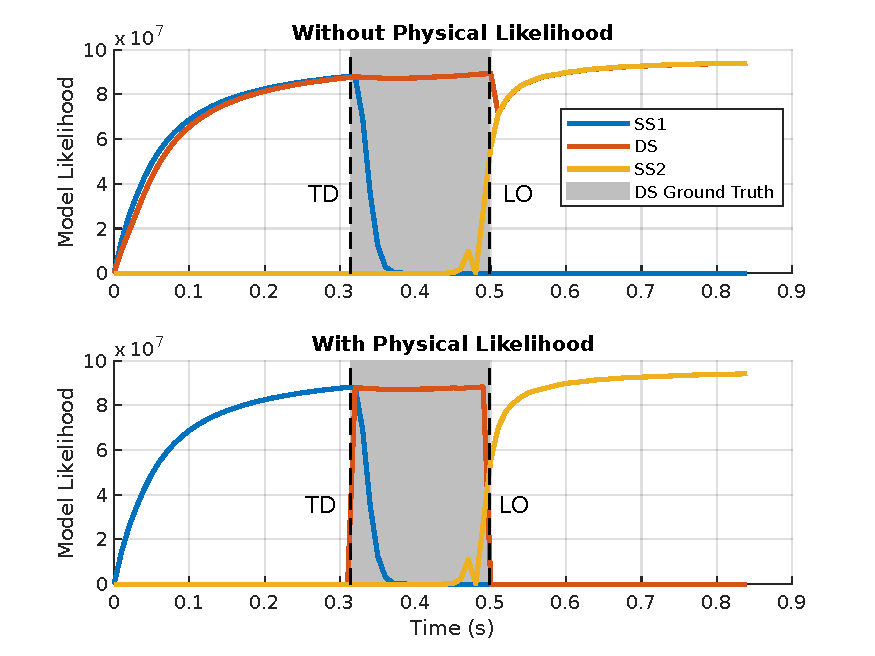
\includegraphics[width=0.7\linewidth]{likeCompare.pdf}
	\caption{The effects of the inclusion of physical likelihood on phase likelihoods}\label{fig:likeCompare}
\end{figure}

A small modification to the conventional IMM was necessary to enable the framework to correctly identify gait modes. 
The likelihood calculation \eqref{eq:likelihood} only looks at the measurement residual, which can be misleading. Dynamics during DS can track the CoM trajectories from SS data by allowing legs to extend beyond their free length, which is not physically possible. A physical likelihood term $ \lambda_p $ was added to the likelihood calculation to address this observation. This strategy takes into account the difference $\Delta l$ between the rest length and current length of the leg, which should remain positive. The likelihood is then modified as
\begin{eqnarray} \label{eq:physicalLikelihood}
	{}^j \ell_k &=& {\rm det}(2 \pi \fsup{\E_k}{j})^{-1/2}\   e^{\lambda_r + \lambda_p}\,,~\textrm{where} \\[.5ex]
	\lambda_p &=& -\kappa \min(0,\Delta l)^2  \nonumber
\end{eqnarray}
and $ \kappa>0$ is a tuning parameter. In DS, the leg with the minimum value for $\Delta l$ is used to compute $\lambda_p$.
This approach decreases the weight of a model if its estimated leg length is greater than its rest length. Figure \ref{fig:likeCompare} shows the effect this modification has on phase inference. With the change, the likelihood of DS only rises during the true DS phase, illustrated with the shaded area. The rate at which the likelihood of DS rises and decays can be tuned using $ \kappa $. With these modifications, the IMM framework can be set up to adequately identify the appropriate dynamics, SS or DS, to be used for state estimation at a given time. This IMM framework was first tested with B-SLIP simulation data and then data acquired from the EksoGT exoskeleton.

\section{Results}
%\begin{figure}
%	\centering
%	\begin{subfigure}{0.5\textwidth}
%		\centering
%		\includegraphics[width=1.1\textwidth]{posEst.pdf} % first figure itself
%		\caption{Position estimates}\label{fig:posEst}
%	\end{subfigure}\hfill
%	\begin{subfigure}{0.5\textwidth}
%		\centering
%		\includegraphics[width=1.1\textwidth]{velEst.pdf}
%		\caption{Velocity estimates}\label{fig:velEst}
%	\end{subfigure}
%	\caption{Position and velocity estimates for exoskeleton data}
%\end{figure}

\subsection{Testing with B-SLIP Simulation Data}

The B-SLIP gait used to generate synthetic measurements was from the library with a forward velocity $ \dot{x}_\com $ = 0.7 m/s. Measurements of the 3D position, forward, and vertical velocity of the CoM in the sagittal plane were used such that $ \y = [x_{\com},\ y_{\com},\ z_{\com},\ \dot{x}_{\com},\ \dot{z}_{\com}]^T $. Zero-mean Gaussian noise with constant covariance $ \R $ was added to the simulated measurements. Process noise was not added to the simulation. However, the process noise covariance $ \Q $ was retained as an estimation parameter as inaccuracies in the dynamics exist when an inaccurate gait/phase is used during estimation. The covariance values used are given by
\begin{align}
	\R &= {\rm diag}([5 ,5 ,5  ,50 ,50]) 
\times 10^{-5} \\
\Q &={\rm diag}([0,0,0,1,1,1])
\times 10^{-2}
\end{align}
where continuous process noise variances for positions and velocities are reported with units m${}^2$/s${}^2$ and m${}^2$/s${}^4$ respectively, and discrete measurement variances for positions and velocities are reported with units m${}^2 $ and m${}^2$/s${}^2$ respectively. 

\begin{figure}
	\centering
	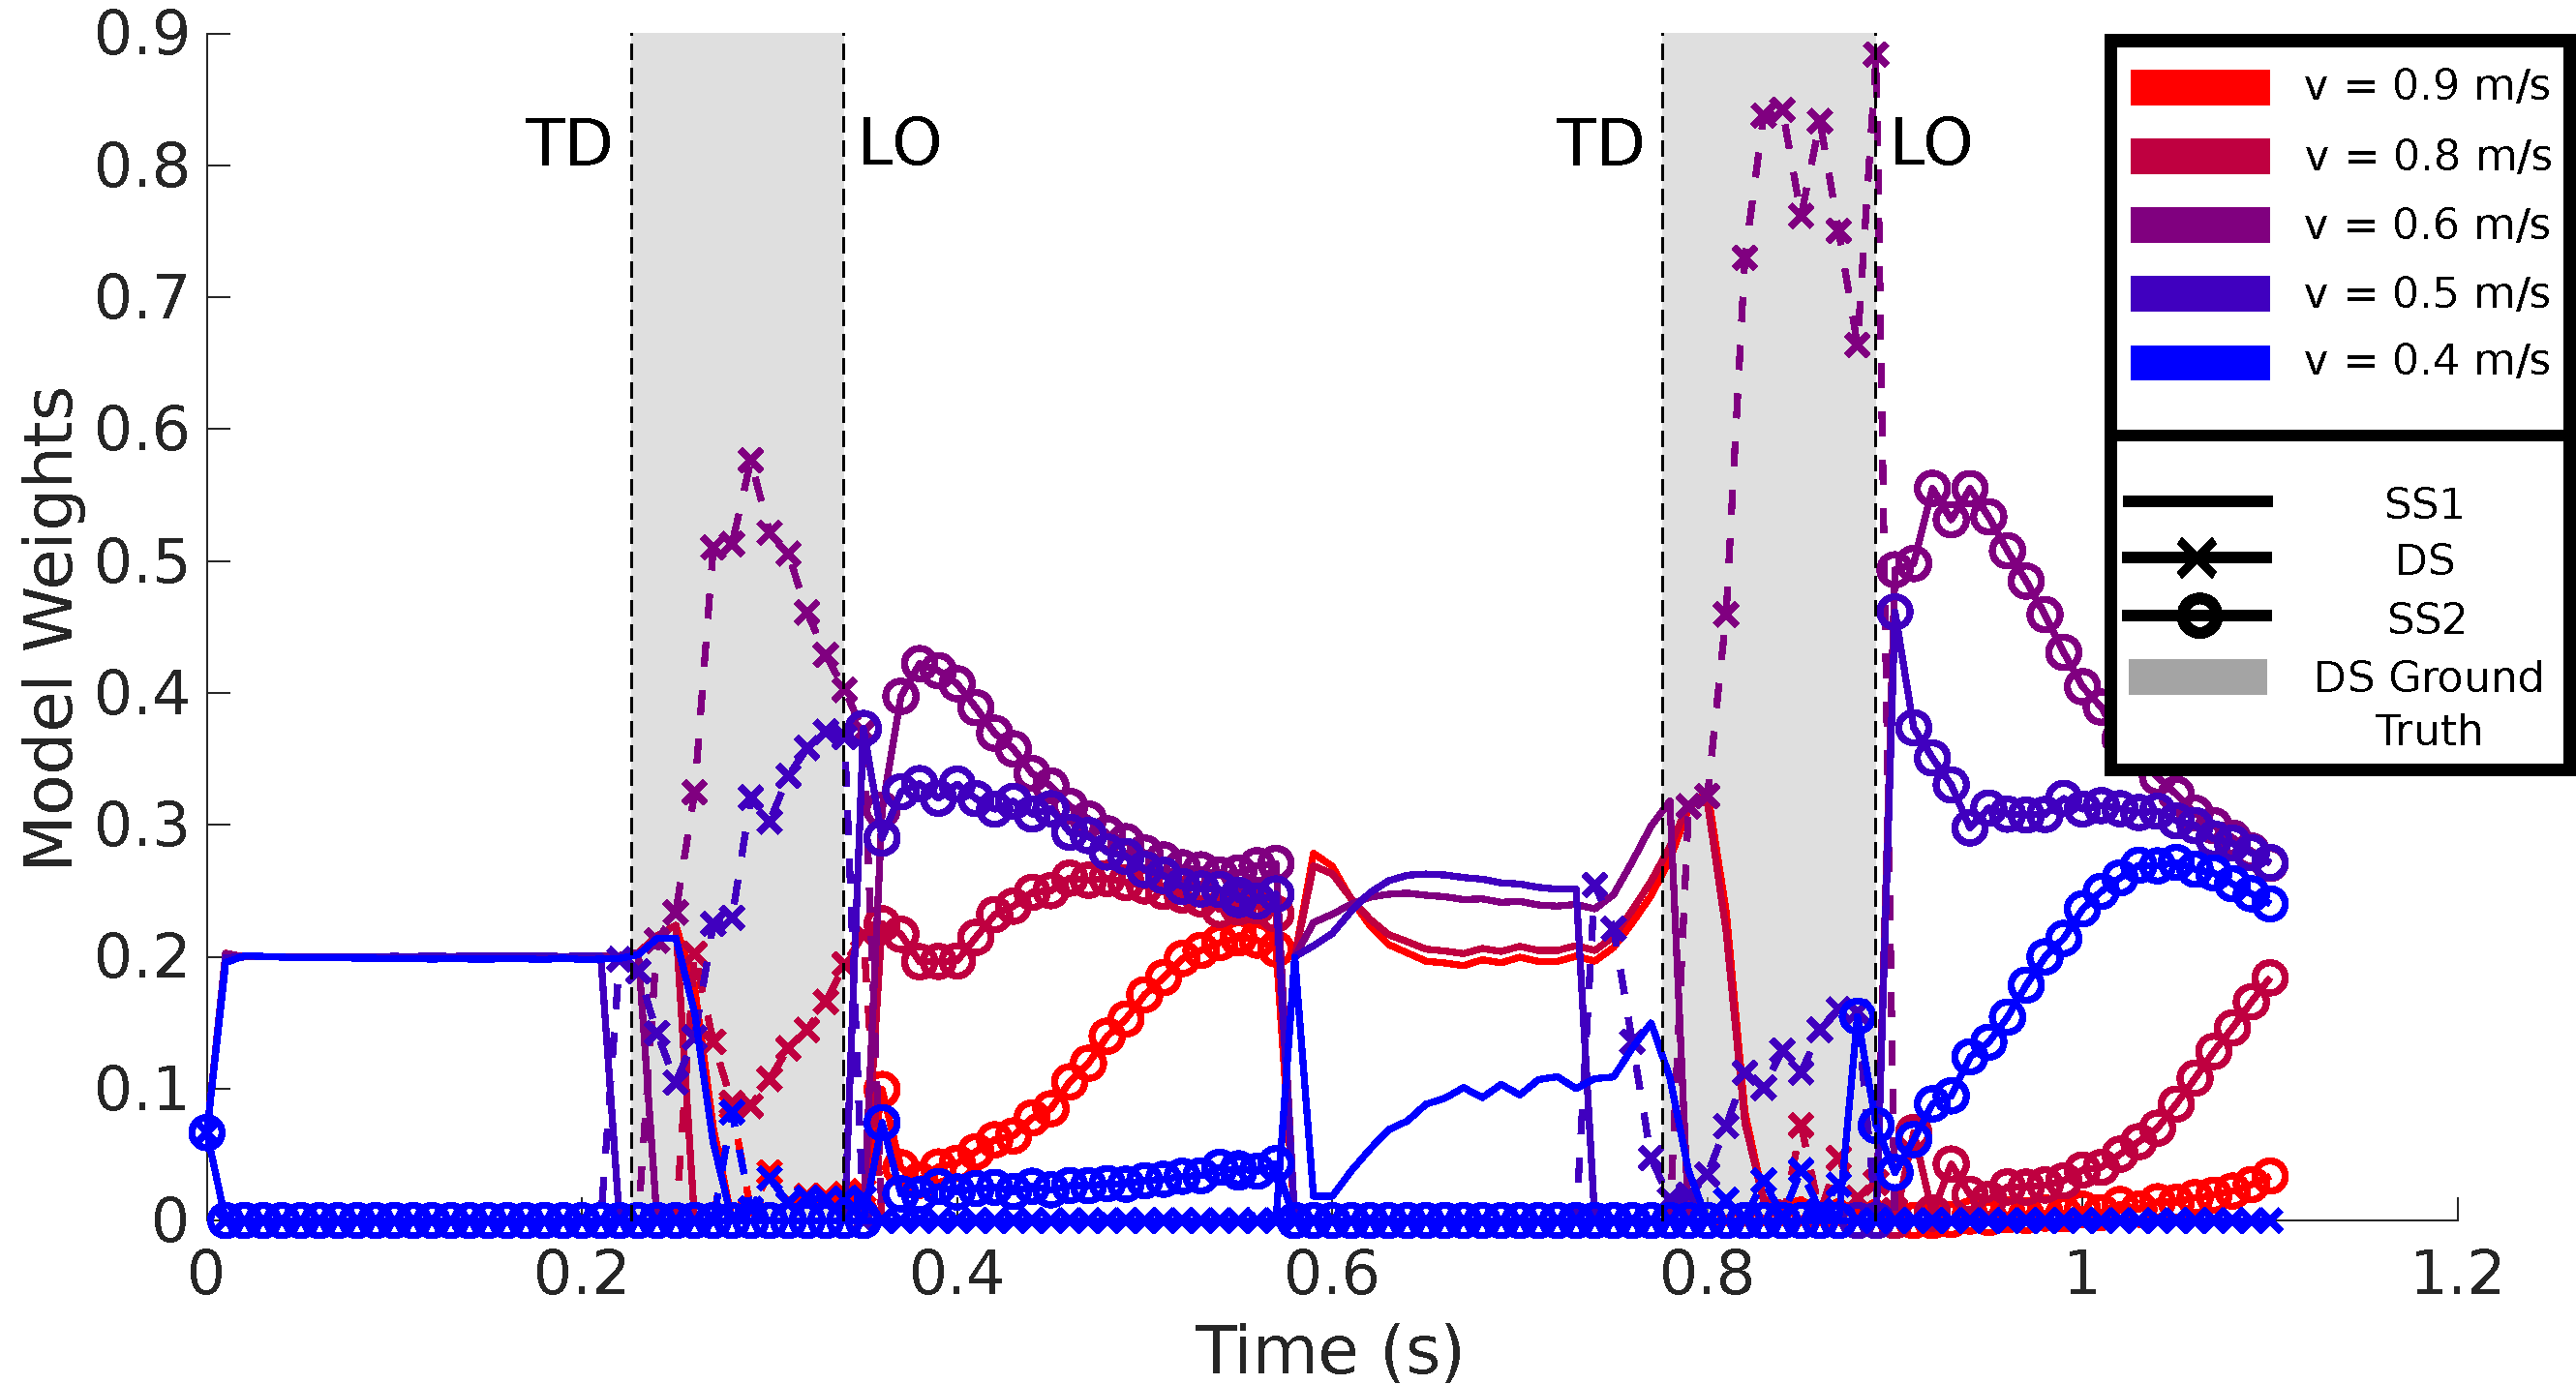
\includegraphics[width=.8\linewidth]{2StepSynth.pdf}
	\caption{Model weights output by the IMM framework applied to measurements generated from a simulation of the B-SLIP model.}\label{fig:weightSyn}
\end{figure}

Figure~\ref{fig:weightSyn} shows the weights associated with each model over two estimations cycles. The gait used to generate the measurements was excluded from the estimation library. The estimator selected the gait at $ \dot{x}_\com $ = 0.6 m/s to be the most likely as the gait that exactly matched the measurements was absent from the library. The CoM trajectories of the library gaits were similar to each other in SS1, therefore the estimator had difficulty distinguishing between them. As the gait progressed through DS, the differences in trajectories became more apparent and the estimator was able to identify the most likely gait. This may be explained by the B-SLIP model's effectiveness at describing the DS gait phase in contrast to rigid pendular models that assume an instantaneous transfer of support.

\subsection{Testing with Exoskeleton Data}

The estimation framework was then tested on data acquired from the sensors onboard the EksoGT exoskeleton during walking trials of an able-bodied person. The subject had a leg length of 0.95 m, weighed 67 kg, and walked at a self-selected speed between 0.6-0.7 m/s using crutches \cite{gambon2019characterizing}. The exoskeleton allows movement only in the sagittal plane and restricts movements in the lateral direction, however, some lateral movement of the CoM is observed due to torso roll. In addition to all the available measurements listed in Sec.~\ref{sec:exoData}, the exoskeleton also reports the estimated height and fore/aft position of the CoM in the global frame. The position of the CoM was approximated and collected in the measurement vector $ \yt = [x_\com ,y_\com ,z_\com]^T $. The evolution of the CoM state of the B-SLIP is sensitive to changes in the leg length of library gaits, particularly in the vertical direction. The parameters that defined the library gaits were rescaled with respect to the estimated CoM height of the exoskeleton user at the initial MS of the estimator trial. Additionally, the following anisotropic process and measurement noise covariances were selected.
\begin{align}
		\R &= {\rm diag}([5,5,0.5])\times 10^{-6} \\
		\Q &={\rm diag}([0,0,0,1,1,10])\times 10^{-2}
\end{align}
This covariance mitigates sensitivity by increasing the estimator's reliance on measurements and decreasing the reliance on the model when inferring vertical CoM evolution. This strategy was found to yield more accurate velocity estimates compared to isotropic covariance selection. 

\begin{figure}
	\centering
	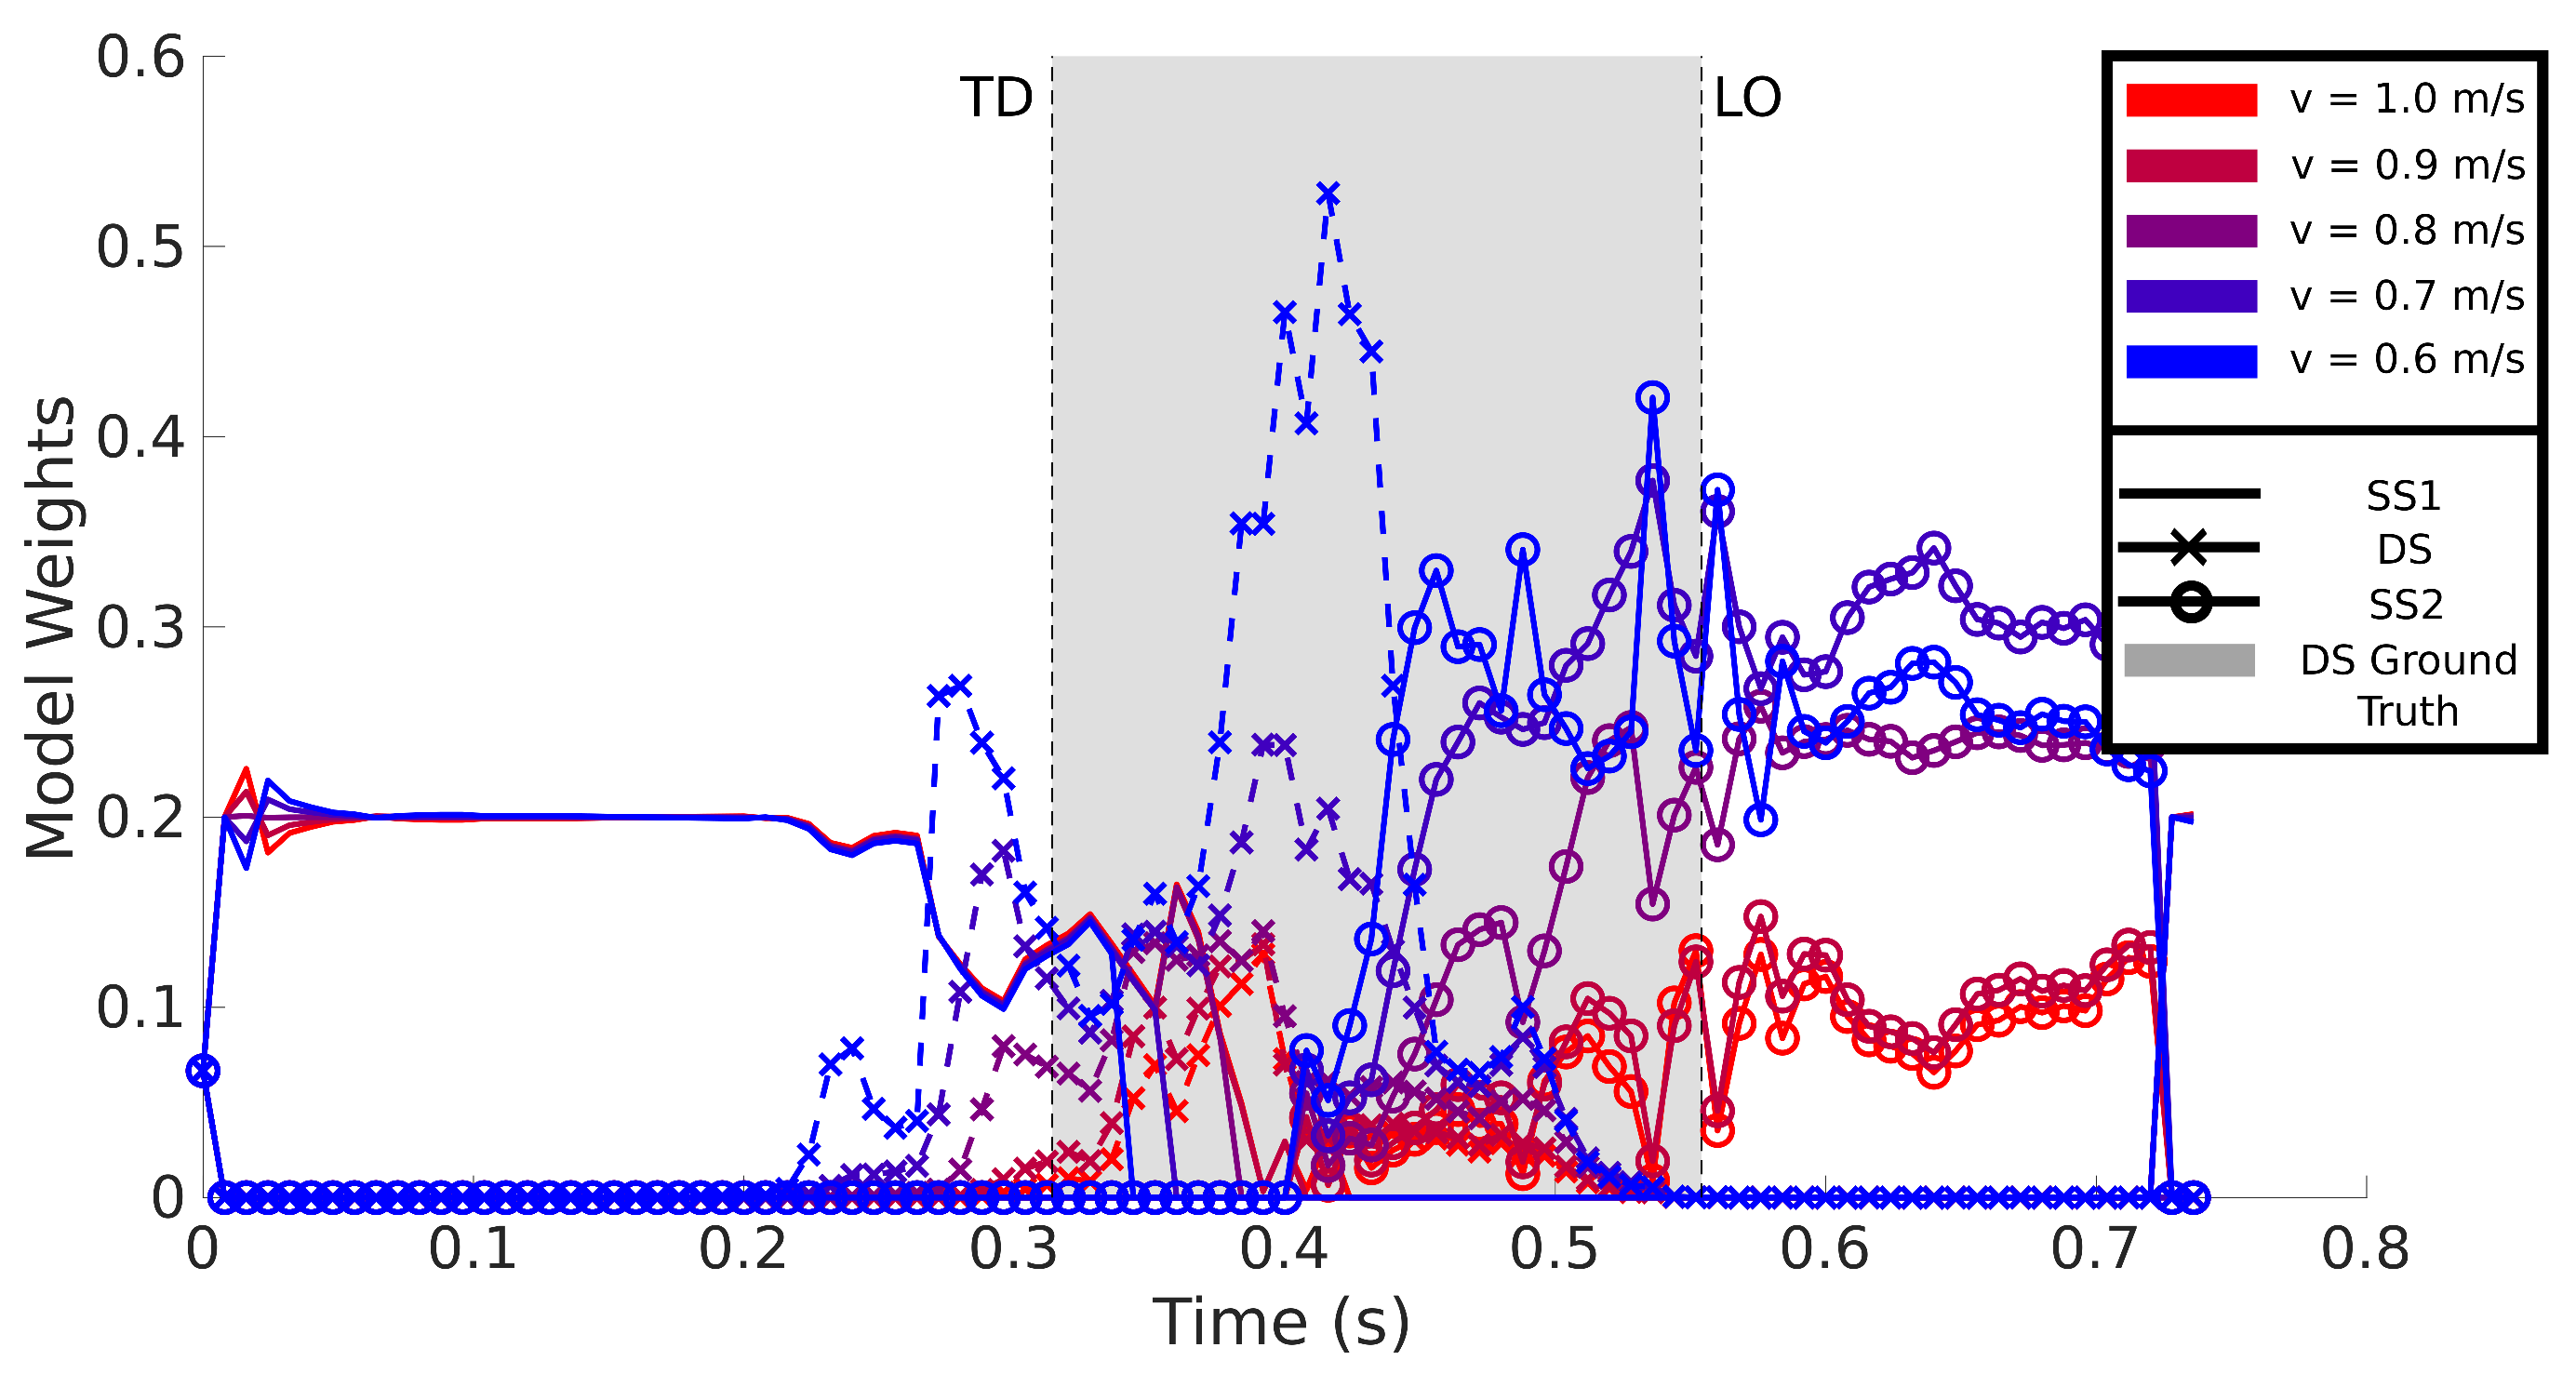
\includegraphics[width=.8\linewidth]{weightsExo.eps}
	\caption{Model weights from the IMM framework applied to experimental measurements of an able-bodied individual walking in an exoskeleton.}\label{fig:exoWeights}
\end{figure}

The most likely gaits for one step of the walking trial are illustrated in Fig.~\ref{fig:exoWeights}; higher weights indicate a more likely gait. The user was walking at a velocity between 0.6-0.7 m/s so the gaits at those speeds are shown to be most likely. All library gaits qualitatively matched human data i.e., maximum forward velocity was achieved during DS, and lateral velocity was zero at the end of the step. However, the initial and lateral positions were optimization variables when generating the gait library, and as a result, they do not match the initial position in the measured data. Therefore estimates of CoM velocities, none of which had direct measurements, took $ \approx $50 m/s to stabilize to expected behavior as illustrated in Fig.~\ref{fig:exoState} where estimates are plotted along with measured values. The DS period, illustrated in gray, was determined when foot-mounted force sensors indicated both feet were flat on the ground.
\begin{figure}
	\centering
	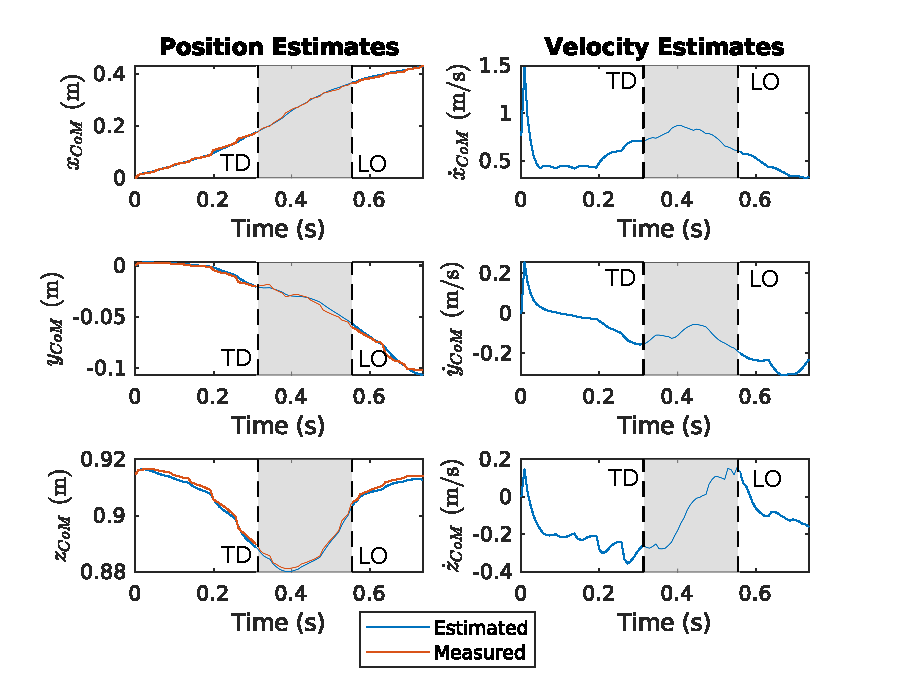
\includegraphics[width= 0.8\linewidth]{stateEstExo.eps}
	\caption{State estimates from the IMM framework applied to experimental measurements of an able-bodied individual walking in an exoskeleton.}\label{fig:exoState}
\end{figure}

\begin{figure}
	\centering
	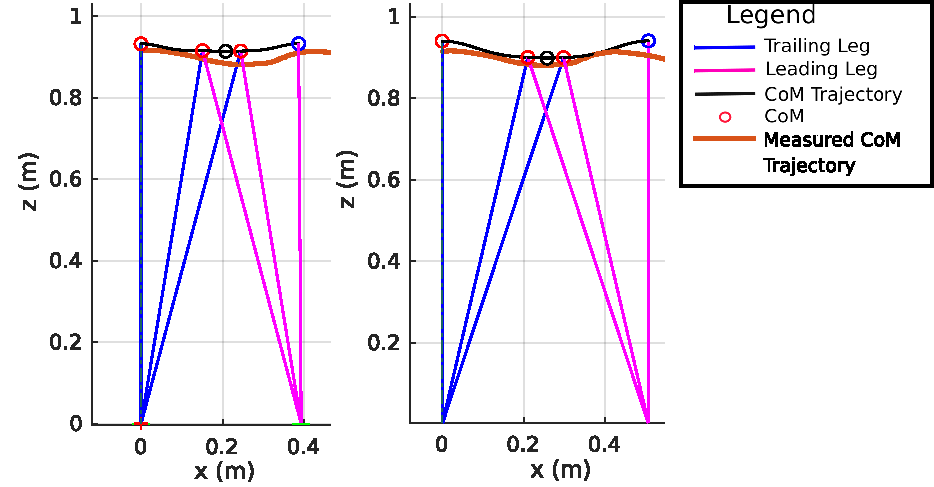
\includegraphics[width=.8\linewidth]{gaitCompare.pdf}
	\caption{Comparison of gaits at speeds of 0.6 m/s  (left) and 1.0 m/s  (right).}\label{fig:compare}
\end{figure}

The estimator relies on differences between measured CoM trajectories and simulated CoM trajectories from library gait to infer gait phase and speed. Figure 10 illustrates that while the exoskeleton user was walking at a speed between 0.6 m/s and 0.7 m/s, the CoM trajectory in the sagittal plane matches more closely with the library gait at a speed of 1.0 m/s as shown in Fig.~\ref{fig:compare}. This behavior may be due to the dynamics of walking in an exoskeleton with an ambulatory device that are not emulated by the B-SLIP model. The IMM framework was able to identify the correct gait velocity and phase of the measured data over a majority of the step despite the mismatch in trajectories. The library contains gaits at 0.6 m/s and 0.7 m/s which are indicated as most likely in Fig.~\ref{fig:exoWeights} as the user's actual gait velocity was between those two values. Thus the IMM framework functions as expected, but relies on accurate emulation of CoM trajectories from library gaits for accurate estimation.

Inaccuracies in the likelihoods of some phases were observed around phase transitions can be seen in Fig.~\ref{fig:weightSyn} and Fig.~\ref{fig:exoWeights}. This behavior is an artifact of the variety of the gait library. Computation of the physical likelihood depends on the leg length, which is the same across all library gaits. However, each of these gaits have different step lengths as the gait velocities are different. As a result, the durations of the DS phases for each of these gaits is also different. Therefore, even with the leg length rescaling, the discrepancy between the human data and library gaits causes the likelihood function to detect DS and infer the end of SS1 at different times, which causes differences in likelihood switching times. The combined state estimates of the CoM positions are still accurate to within 1cm of the measurements despite this (Fig.~\ref{fig:exoState}).

\section{Challenges with using IMMs}

\begin{figure}
	\centering
	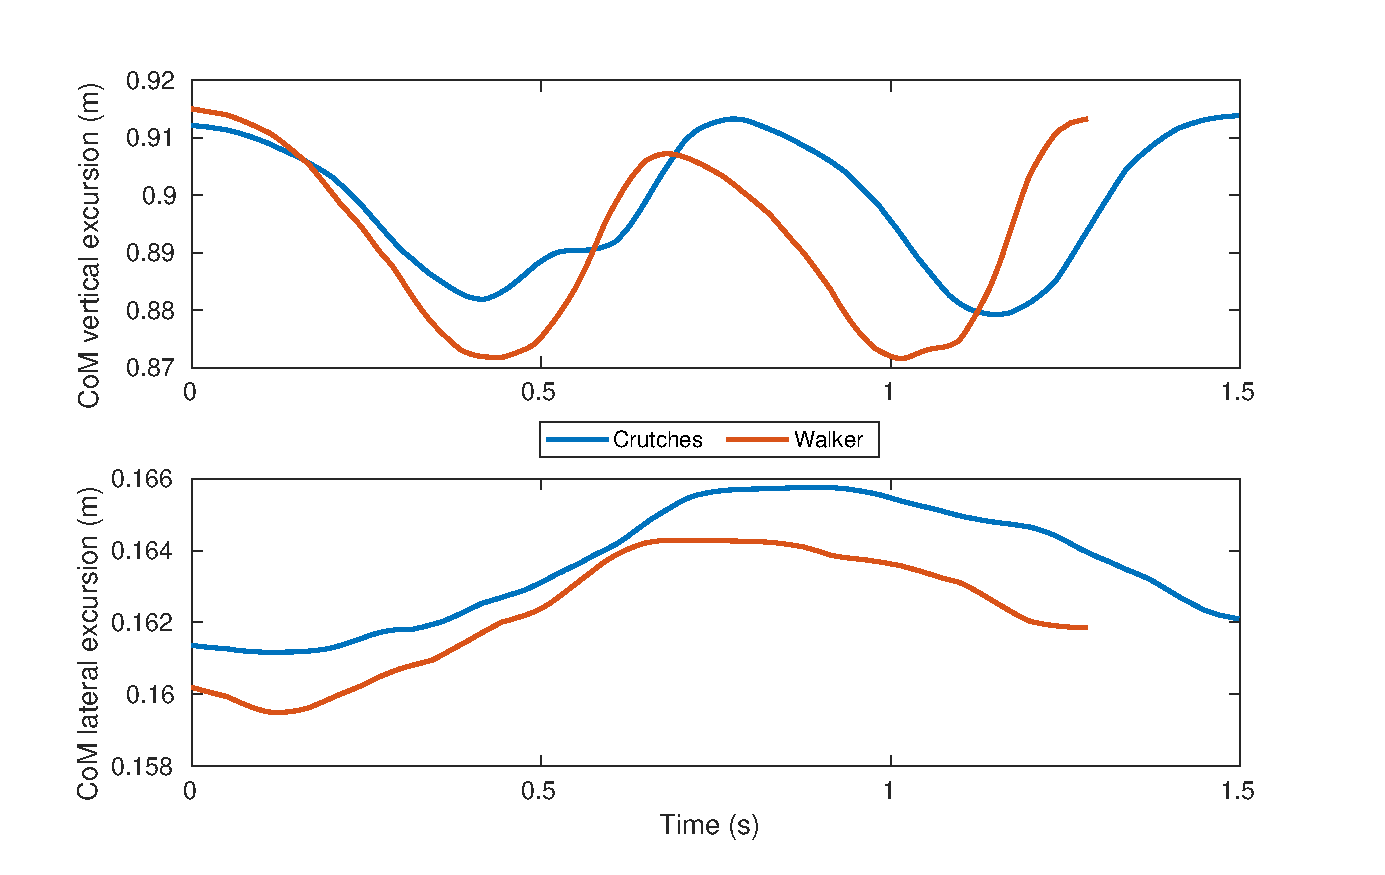
\includegraphics[width=0.8\linewidth]{trajDiff}
	\caption{CoM trajectories for two steps of the same subject walking at steady-state with a self-selected gait speed using a walker vs. crutches.}\label{fig:trajDiff}
\end{figure}
Discrepancies were observed between the measured CoM trajectories and those of B-SLIP gaits. The measured CoM trajectories are asymmetric and it is difficult to generate high-fidelity matching B-SLIP gaits. Center of mass trajectories are influenced by a variety of factors such as the choice of ambulatory device, and gait features such as gait speed, and individual joint trajectories resulting from uncoordinated limb movements. Figure~\ref{fig:trajDiff} shows the CoM trajectories of the same subject over two steps walking at steady-state using a walker and crutches. The step length and therefore, step duration, were shorter when the walker was being used resulting in considerably different trajectories. This variation in trajectories is challenging to capture using only the B-SLIP model and simply increasing the number of gaits considered by the IMM is an insufficient solution.

The ensemble estimate as calculated by the IMM (Eq.~\ref{eq:estimates}) is a weighted summation of estimates from the filter library. As all gaits in the gait library are intended to match human walking, the likelihoods of the corresponding estimates will rarely go to zero. Therefore, the more gaits there are in the library, the more "polluted" the ensemble estimate will be due to irrelevant estimates being included. The implementation of the physical likelihood in Eq.~\ref{eq:physicalLikelihood} mitigates this issue between gait phases, but it does not address this issue when dealing with different filters of the same phase. A similar problem of context-based estimator selection and its scalability was addressed for legged robots by deactivating and reactivating individual filters \cite{skaff2010context} based on measurements from sensors onboard the robot. However, this approach may not capture the variability observed in human walking.

\section{Conclusion}
In conclusion, the IMM framework is capable of estimating an exoskeleton user's intended gait and phase by comparing measured CoM trajectories of exoskeleton users to simulated B-SLIP gaits. The  quality of these estimates is highly dependent on the quality of the underlying gait library as the estimation relies solely on matching CoM trajectories. Changes in the individual gait variables add up to influence CoM trajectory. It may not always be possible to predict these changes with a simple template model such as the B-SLIP, therefore, the IMM framework may be used as a high-level framework that may be supplemented by another estimator to monitor the individual gait features that affect CoM trajectories. The reactive nature of this framework may also be addressed by considering these gait features and relating them to changes in gait velocity.